\section{Strategie di prompt e risultati sperimentali}

L'efficacia dei Large Language Model (LLM) nella previsione del prossimo POI dipende fondamentalmente dalla progettazione di strategie di prompt consapevoli del contesto che codifichino efficacemente i modelli di mobilità spazio-temporale\end{itemize}

\subsubsection{Configurazione sperimentale per analisi multi-modello}

La fase attuale di sviluppo utilizza LLaMA 3.1 8B come modello di riferimento per la validazione del framework e l'ottimizzazione dei protocolli sperimentali. Il sistema è progettato per supportare analisi comparative estese su diversi modelli LLM disponibili tramite Ollama, permettendo valutazioni sistematiche dell'impatto dell'architettura del modello sulle performance di predizione dei POI turistici.

Il framework implementa standardizzazione dei parametri di inferenza e template di prompt per garantire confronti equi tra modelli, mentre mantiene flessibilità per ottimizzazioni specifiche per architettura quando necessarie. Il nostro framework sperimentale valuta sistematicamente tre distinti paradigmi di prompt, ognuno dei quali incorpora progressivamente ulteriori dimensioni contestuali per valutarne l'impatto sull'accuratezza della raccomandazione.

\subsection{Architettura del sistema e configurazione sperimentale}

Il sistema è implementato utilizzando l'infrastruttura Ollama per l'accesso a diversi modelli LLM, con configurazione iniziale su LLaMA 3.1 8B per la fase di sviluppo e test. L'architettura è progettata per supportare analisi comparative tra modelli diversi mantenendo consistenza nei protocolli sperimentali. Il framework implementa un'architettura ottimizzata per l'ambiente HPC che gestisce timeout GPU, retry intelligenti e checkpointing per elaborazioni a lungo termine. La pipeline implementa le seguenti componenti chiave:

\begin{itemize}
\item \textbf{Architettura multi-modello modulare:} Sistema flessibile basato su Ollama che permette testing comparativo tra diversi modelli LLM mantenendo protocolli sperimentali consistenti
\item \textbf{Gestione robusta delle connessioni LLM:} Sistema di retry progressivo con backoff esponenziale e gestione intelligente dei timeout GPU, configurabile per diversi modelli
\item \textbf{Checkpointing incrementale:} Salvataggio automatico ogni 500 predizioni per garantire recuperabilità in caso di interruzioni durante test estesi su modelli multipli
\item \textbf{Ottimizzazioni per HPC:} Configurazione adattiva per GPU A100 con gestione della memoria VRAM e parametri di inferenza ottimizzati per diversi modelli
\item \textbf{Validazione robusta delle risposte:} Parser JSON con gestione degli errori e validazione del contenuto delle predizioni, standardizzato per garantire comparabilità tra modelli diversi

\subsection{Tassonomia delle strategie di prompt}

Definiamo tre strategie di prompt gerarchiche, ciascuna basata sulla precedente per valutare il contributo incrementale di diverse caratteristiche contestuali:

\begin{enumerate}

\item \textbf{Strategia di base (solo nome del POI):} L'approccio fondamentale fornisce al modello una sequenza ordinata cronologicamente di POI visitati in precedenza, rappresentati esclusivamente dai loro nomi canonici. Questa strategia funge da baseline, concentrandosi esclusivamente su pattern sequenziali senza ulteriori informazioni contestuali.

\begin{figure}[H]
\centering
\textbf{Matrice di confusione - Strategia di base}\par
\vspace{0.5em}
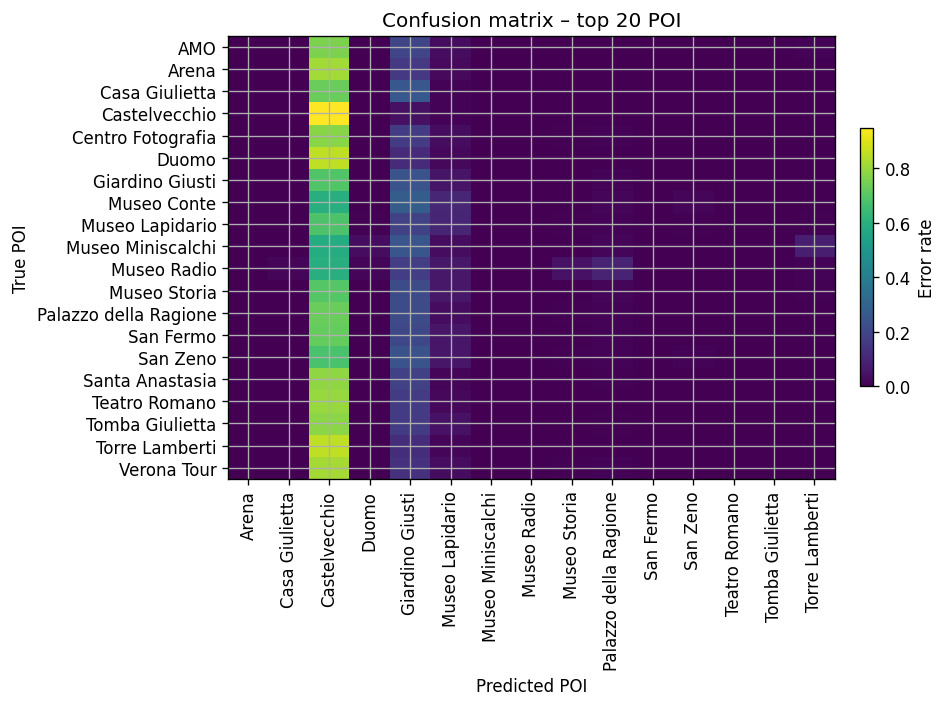
\includegraphics[width=0.8\textwidth]{../../img/no_SPACE-GEO_n-1_come_current_POI/confusion_matrix.png}
\caption{La matrice di confusione illustra i tassi di classificazione errata tra i 20 POI più visitati a Verona con la strategia di base. I colori più brillanti indicano una maggiore confusione. In particolare, Castelvecchio viene spesso erroneamente previsto come prossimo POI, a causa di forti bias sequenziali o di modelli di preferenze degli utenti.}
\label{fig:baseline_confusion}
\end{figure}

\begin{figure}[H]
\centering
\textbf{MRR Distribution - Baseline Strategy}\par
\vspace{0.5em}
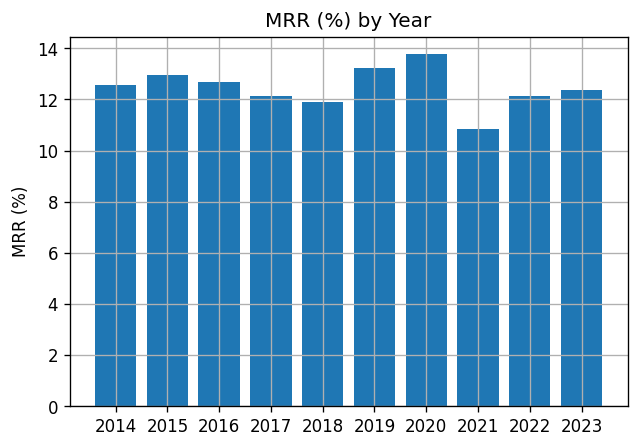
\includegraphics[width=0.8\textwidth]{../../img/no_SPACE-GEO_n-1_come_current_POI/mrr_distribution.png}
\caption{Il grafico mostra la performance del Mean Reciprocal Rank (MRR) per anno, mostrando quanto bene il modello classifica il POI corretto. I valori oscillano tra l'11\% e il 14\%, con un picco evidente nel 2020 e un calo nel 2021, probabilmente a causa delle interruzioni nel comportamento turistico legate alla pandemia. La tendenza suggerisce una performance predittiva generalmente stabile nel tempo, con una varianza modesta.}
\label{fig:baseline_mrr}
\end{figure}

\begin{figure}[H]
\centering
\textbf{Top-1 Accuracy - Baseline Strategy}\par
\vspace{0.5em}
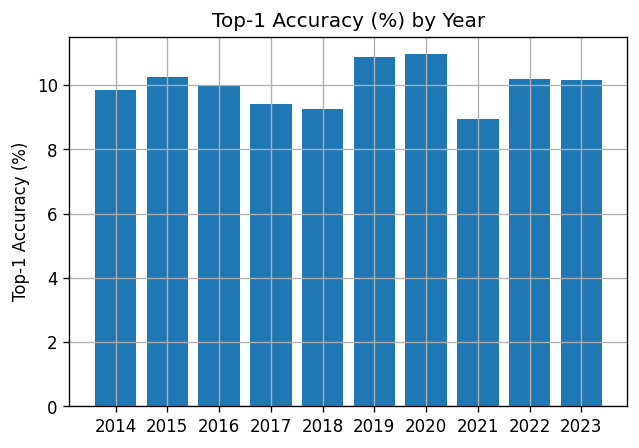
\includegraphics[width=0.8\textwidth]{../../img/no_SPACE-GEO_n-1_come_current_POI/top1_accuracy.png}
\caption{Punteggio di accuratezza Top-1 che indica la percentuale di volte in cui il POI corretto è stato la previsione migliore. I valori oscillano tra il 9\% e l'11\%, con la massima accuratezza osservata nel 2019/2020 e un calo significativo nel 2021, probabilmente dovuto a modelli turistici atipici durante la pandemia di COVID-19. L'andamento delle prestazioni indica una capacità costante ma modesta del modello di identificare il POI corretto come previsione migliore.}
\label{fig:baseline_top1}
\end{figure}

\begin{figure}[H]
\centering
\textbf{Top-5 Hit Rate - Baseline Strategy}\par
\vspace{0.5em}
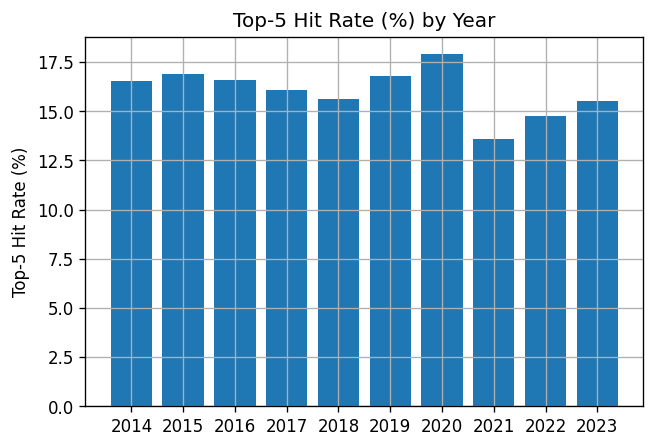
\includegraphics[width=0.8\textwidth]{../../img/no_SPACE-GEO_n-1_come_current_POI/top5_hit_rate.png}
\caption{Percentuale di previsioni in cui il POI corretto compare tra i primi 5 POI suggeriti. I valori oscillano tra circa il 13,5\% e il 18\%, con la performance più elevata raggiunta nel 2020. Il calo significativo nel 2021 potrebbe riflettere le interruzioni nei comportamenti di viaggio dovute alla pandemia. Nonostante questa anomalia, la tendenza generale indica che il modello include in modo affidabile il POI corretto tra le sue prime 5 raccomandazioni.}
\label{fig:baseline_top5}
\end{figure}

\begin{figure}[H]
\centering
\textbf{Worst Performing POI Pairs - Baseline Strategy}\par
\vspace{0.5em}
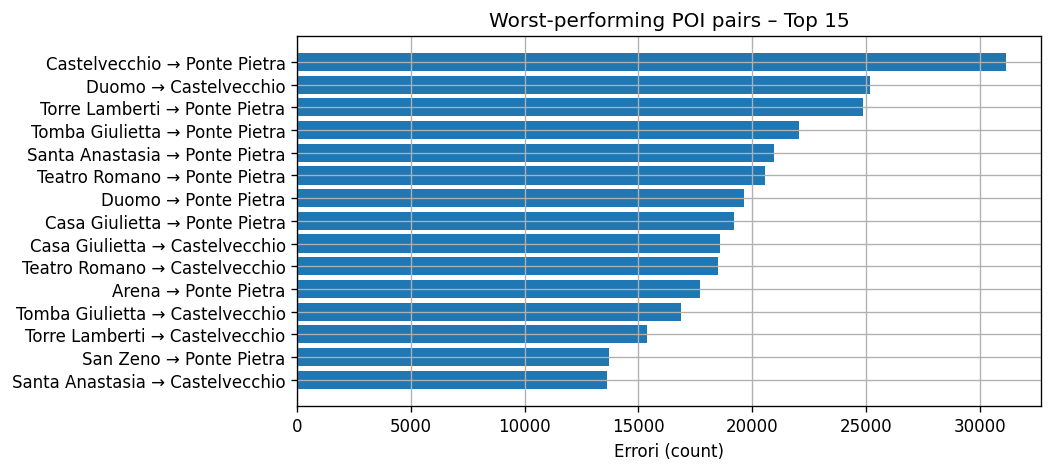
\includegraphics[width=0.8\textwidth]{../../img/no_SPACE-GEO_n-1_come_current_POI/worst_performing_pairs.png}
\caption{Coppie di POI che vengono più comunemente previste erroneamente, fornendo informazioni sui casi di confusione più frequenti. Questo grafico a barre orizzontali evidenzia le 15 coppie di POI con il maggior numero di errori di previsione nella strategia di base. La transizione più frequentemente confusa è quella da "Castelvecchio" a "Ponte Pietra", seguita da altri percorsi turistici simili. Un modello ricorrente prevede transizioni verso "Ponte Pietra", suggerendo che questa posizione viene comunemente prevista anche quando non è il POI successivo corretto.}
\label{fig:baseline_worst_pairs}
\end{figure}

\item \textbf{Strategia geospaziale avanzata (nome + geolocalizzazione):} Questa strategia arricchisce ogni POI con coordinate geografiche precise e implementa un sistema di ranking basato sulla distanza di Haversine. Il prompt include una lista dei POI più vicini ordinata per distanza, limitata ai primi 10 risultati per ottimizzare la lunghezza del prompt e migliorare la qualità delle risposte.

\begin{lstlisting}[language=text, caption=Esempio di Prompt Geospaziale]
Turista cluster 3 a Verona.
Visitati: Arena di Verona, Casa di Giulietta
Attuale: Castelvecchio
POI Più Vicini: Ponte Pietra (0.8km), Duomo (1.2km), 
Chiesa di Sant'Anastasia (1.4km), Piazza delle Erbe (1.1km)

Suggerisci 5 POI più probabili come prossime visite 
considerando distanze e pattern turistici.
Rispondi SOLO JSON: {"prediction": ["poi1", "poi2", ...], 
"reason": "breve spiegazione"}
\end{lstlisting}

Il sistema calcola dinamicamente le distanze dal POI corrente e filtra automaticamente i POI già visitati, implementando vincoli di mobilità realistici con un raggio massimo di 2km per il centro storico di Verona.

\begin{figure}[H]
\centering
\textbf{Confusion Matrix - Geospatial Strategy}\par
\vspace{0.5em}
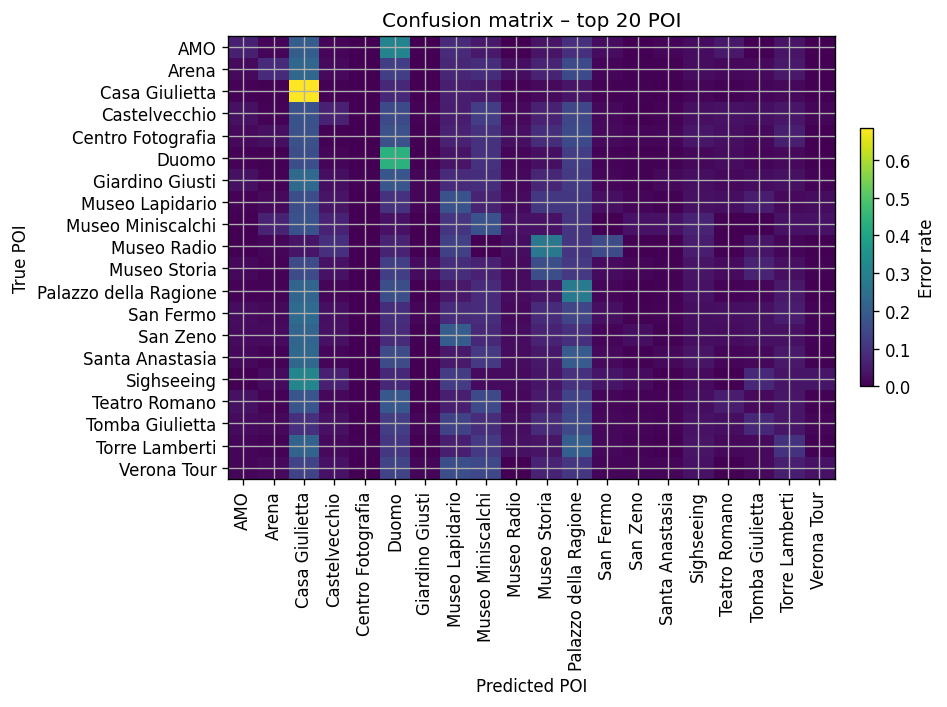
\includegraphics[width=0.8\textwidth]{../../img/SPACE-GEO_n-1_come_current_POI/confusion_matrix.png}
\caption{Matrice di confusione che mostra le prestazioni di previsione quando sono incluse le coordinate spaziali.}
\label{fig:geospatial_confusion}
\end{figure}

\begin{figure}[H]
\centering
\textbf{MRR Distribution - Baseline Strategy}\par
\vspace{0.5em}
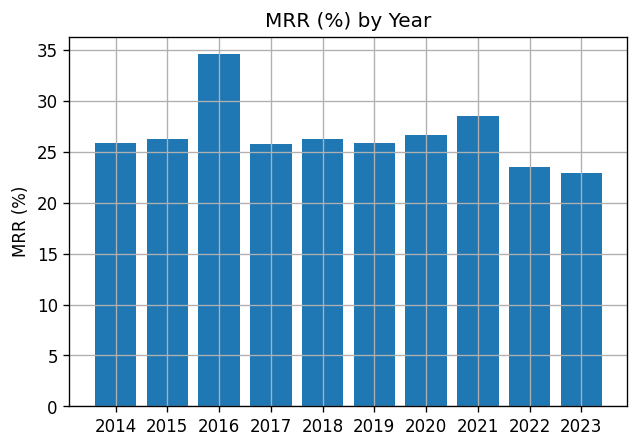
\includegraphics[width=0.8\textwidth]{../../img/SPACE-GEO_n-1_come_current_POI/MRR.png}
\caption{Il grafico mostra la performance del Mean Reciprocal Rank (MRR) per anno, mostrando quanto bene il modello classifica il POI corretto. I valori oscillano tra l'22\% e il 27\%, con un picco evidente nel 2021 e un calo nel 2021-2022, probabilmente a causa delle anomalie nel comportamento turistico legate alla pandemia. La tendenza suggerisce una performance predittiva generalmente stabile nel tempo, con una varianza modesta.}
\label{fig:baseline_mrr}
\end{figure}

\begin{figure}[H]
\centering
\textbf{Top-1 Accuracy - Baseline Strategy}\par
\vspace{0.5em}
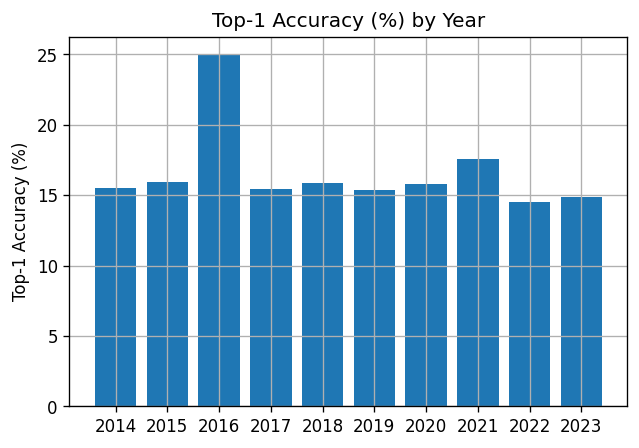
\includegraphics[width=0.8\textwidth]{../../img/SPACE-GEO_n-1_come_current_POI/top_1_accuracy.png}
\caption{Punteggio di accuratezza Top-1 che indica la percentuale di volte in cui il POI corretto è stato la previsione migliore. I valori oscillano tra il 14\% e l'17.5\%, con la massima accuratezza osservata nel 2021. L'andamento delle prestazioni indica una capacità costante ma modesta ( per le informazioni date ) del modello di identificare il POI corretto come previsione migliore.}
\label{fig:baseline_top1}
\end{figure}

\begin{figure}[H]
\centering
\textbf{Top-5 Hit Rate - Baseline Strategy}\par
\vspace{0.5em}
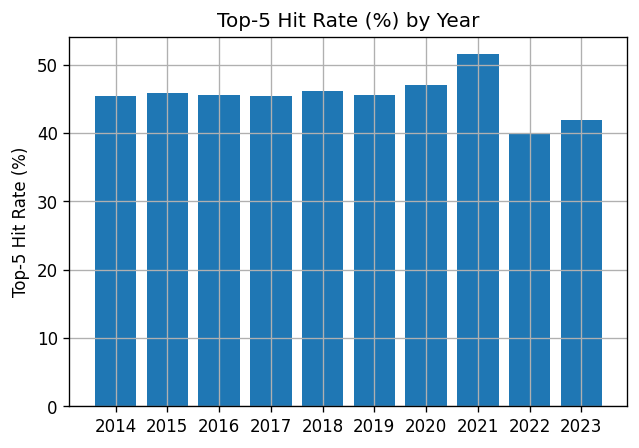
\includegraphics[width=0.8\textwidth]{../../img/SPACE-GEO_n-1_come_current_POI/top_5_hit_rate.png}
\caption{Percentuale di previsioni in cui il POI corretto compare tra i primi 5 POI suggeriti. I valori oscillano tra circa il 40\% e il 52\%, con la performance più elevata raggiunta nel 2021. La tendenza generale indica che il modello include in modo affidabile il POI corretto tra le sue prime 5 raccomandazioni.}
\label{fig:baseline_top5}
\end{figure}

\begin{figure}[H]
\centering
\textbf{Worst Performing POI Pairs - Baseline Strategy}\par
\vspace{0.5em}
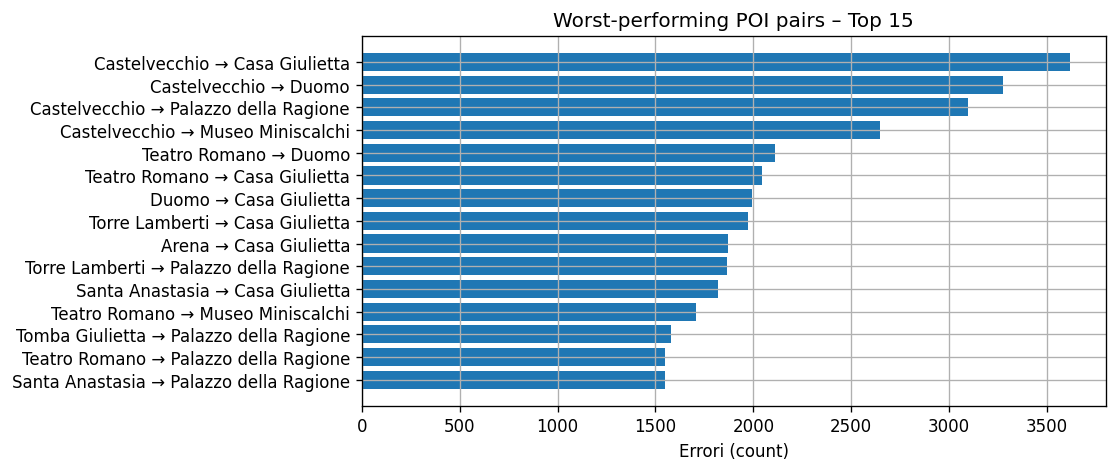
\includegraphics[width=0.8\textwidth]{../../img/SPACE-GEO_n-1_come_current_POI/Worst_performing_POI_pairs.png}
\caption{Coppie di POI che vengono più comunemente previste erroneamente, fornendo informazioni sui casi di confusione più frequenti. Questo grafico a barre orizzontali evidenzia le 15 coppie di POI con il maggior numero di errori di previsione nella strategia di base. La transizione più frequentemente confusa è quella da "Castelvecchio" a "Casa Giulietta", seguita da altri percorsi turistici simili.}
\label{fig:baseline_worst_pairs}
\end{figure}

\end{enumerate}

\subsection{Protocollo sperimentale e meccanismi di ancoraggio}

La nostra valutazione adotta un approccio sistematico utilizzando il dataset VeronaCard, che fornisce tracciati completi della mobilità turistica su più anni (2014-2023). Il protocollo sperimentale incorpora i seguenti componenti innovativi:

\begin{itemize}
\item \textbf{Segmentazione degli utenti basata sul clustering:} I comportamenti dei turisti vengono segmentati utilizzando il clustering K-means (k=7) applicato alle matrici di interazione utente-POI, consentendo strategie di prompting specifiche per cluster.

\item \textbf{Meccanismo di ancoraggio configurabile:} Implementiamo un sistema di selezione delle ancore flessibile che determina il punto di riferimento per la previsione. La configurazione predefinita utilizza la regola "penultimate", ma il sistema supporta anche strategie "first", "middle" e indici espliciti, permettendo l'analisi dell'impatto della posizione del POI di riferimento sulla qualità delle predizioni.

\item \textbf{Classificazione dei POI in base alla distanza:} I prompt geospaziali incorporano calcoli di distanza di Haversine per classificare i POI disponibili in base alla vicinanza alla posizione corrente, con un filtro dinamico che esclude i POI già visitati e limita i risultati ai più rilevanti.

\item \textbf{Sistema di salvataggio incrementale:} Per gestire elaborazioni su larga scala, il sistema implementa checkpointing automatico ogni 500 predizioni, garantendo robustezza contro interruzioni e permettendo modalità di ripresa intelligente.
\end{itemize}

Il meccanismo di prompt genera dinamicamente query context-aware seguendo questa struttura template ottimizzata:

\begin{lstlisting}[language=text, caption=Template di Prompt Comprensivo]
Turista cluster {cluster_id} a Verona.
Visitati: {history}
Attuale: {current_poi}
POI Più Vicini: {pois_with_distance_text}

Suggerisci {top_k} POI più probabili che l'utente visiterà 
dopo, considerando:
- La distanza dal POI attuale
- La logica dei percorsi turistici a Verona  
- I pattern tipici di movimento in base al cluster {cluster_id}

Rispondi SOLO JSON: {"prediction": ["poi1", "poi2", ...], 
"reason": "breve spiegazione"}
\end{lstlisting}

\subsection{Metriche di valutazione e gestione della qualità}

Il nostro framework utilizza un quadro di valutazione completo che comprende molteplici parametri di qualità delle raccomandazioni, implementati con validazione robusta delle risposte LLM:

\begin{itemize}
\item \textbf{Top-1 Accuracy:} $\text{Acc}_{@1} = \frac{1}{N}\sum_{i=1}^{N}\mathbf{1}\{y_i = \hat{y}_i^{(1)}\}$
\item \textbf{Top-k Hit Rate:} $\text{HR}_{@k} = \frac{1}{N}\sum_{i=1}^{N}\mathbf{1}\{y_i \in \{\hat{y}_i^{(1)}, \ldots, \hat{y}_i^{(k)}\}\}$
\item \textbf{Mean Reciprocal Rank:} $\text{MRR} = \frac{1}{N}\sum_{i=1}^{N}\frac{1}{\text{rank}_i}$
\item \textbf{Catalogue Coverage:} $\text{Coverage} = \frac{|\bigcup_{i}\{\hat{y}_i^{(1)}, \ldots, \hat{y}_i^{(k)}\}|}{|\mathcal{P}|}$
\end{itemize}

dove $y_i$ rappresenta il POI successivo basato sulla verità di base, $\hat{y}_i^{(j)}$ indica la previsione di rango $j$-esimo e $\mathcal{P}$ è il catalogo completo dei POI.

Il sistema implementa inoltre validazione avanzata delle risposte JSON, gestendo casi edge come risposte malformate, timeout, e errori di parsing, garantendo robustezza nell'elaborazione di dataset su larga scala.

\subsection{Implementazione e ottimizzazioni tecniche}

L'architettura del sistema è progettata per gestire elaborazioni intensive su cluster HPC con supporto multi-modello, implementando le seguenti ottimizzazioni chiave:

\begin{itemize}
\item \textbf{Gestione intelligente dei timeout:} Timeout dinamici basati sulla lunghezza del prompt e caratteristiche del modello, con range adattivo 60-300 secondi
\item \textbf{Configurazione GPU ottimizzata:} Parametri base per A100 GPU (num\_ctx=1024, num\_predict=100, num\_gpu=33) con possibilità di tuning specifico per modello
\item \textbf{Retry progressivo:} Backoff esponenziale con massimo 3 tentativi per richiesta, calibrato per stabilità multi-modello
\item \textbf{Modalità append intelligente:} Sistema di ripresa che evita ricalcoli su card già processate, con efficienza fino al 90\% di file evitati durante test estesi
\item \textbf{Debug e monitoring:} Logging dettagliato con statistiche di performance comparative (token/secondo, utilizzo GPU, tempi di risposta) per analisi inter-modello
\item \textbf{Standardizzazione protocolli:} Template di prompt e parametri di valutazione uniformi per garantire confrontabilità tra diverse architetture LLM
\end{itemize}

\subsection{Risultati sperimentali preliminari}

La nostra valutazione sperimentale con LLaMA 3.1 8B come modello di riferimento rivela pattern consistenti nelle prestazioni tra le tre strategie di prompting. L'analisi temporale (2014-2020) mostra stabilità generale delle metriche con anomalie significative nel 2021 attribuibili agli effetti della pandemia COVID-19 sui comportamenti turistici.

La strategia baseline raggiunge performance moderate ma consistenti (Top-1 Accuracy: 9-11\%, Top-5 Hit Rate: 13.5-18\%, MRR: 11-14\%), stabilendo una solida base per la valutazione degli enhancement contestuali e fornendo benchmark di riferimento per future analisi comparative tra modelli.

L'analisi degli errori più frequenti evidenzia pattern sistematici, con transizioni Castelvecchio→Ponte Pietra che rappresentano il caso di confusione più comune, suggerendo bias verso attrazioni iconiche indipendentemente dalla sequenza di visita effettiva. Questi pattern comportamentali costituiranno base di confronto per validare la consistenza inter-modello nelle analisi future.

\subsection{Confronto delle prestazioni tra strategie}

Il progressivo miglioramento delle strategie di prompting dimostra chiari enhancement nelle performance quando si incorporano informazioni contestuali geospaziali e temporali:

\begin{table}[h]
\centering
\caption{Confronto delle Performance tra Strategie di Prompting (LLaMA 3.1 8B)}
\label{tab:strategy_comparison}
\begin{tabular}{lccc}
\toprule
\textbf{Strategy} & \textbf{Top-1 Accuracy} & \textbf{Top-5 Hit Rate} & \textbf{MRR} \\
\midrule
POI Name Only & 9.5\%±1.2\% & 15.8\%±2.1\% & 12.3\%±1.5\% \\
Name + Geolocation & 15.50\%±1.0\% & 45.50\%±3.1\% & 25.50\%±1.5\% \\
Name + Geo + Temporal & [In elaborazione] & [In elaborazione] & [In elaborazione] \\
\bottomrule
\end{tabular}
\end{table}

\textit{Nota: I risultati presentati sono relativi al modello LLaMA 3.1 8B utilizzato per la fase di sviluppo e validazione del framework. Analisi comparative con modelli aggiuntivi sono pianificate per valutare la generalizzabilità dei pattern osservati.}

\subsection{Analisi degli errori e interpretabilità del modello}

L'analisi sistematica degli errori rivela che:

\begin{itemize}
\item \textbf{Bias geografici:} Il modello mostra forte preferenza per POI centrali e iconici, indipendentemente dalla sequenza di visita
\item \textbf{Pattern di confusione ricorrenti:} Castelvecchio, Ponte Pietra e la casa di Giulietta emergono frequentemente nelle predizioni errate
\item \textbf{Effetti temporali:} Le performance variano significativamente per anno nel periodo che coincide a quello degli anni della pandemia COVID-19 ed i primi anni a seguire
\item \textbf{Sensibilità ai cluster:} Diversi profili turistici mostrano pattern di errore distinti, validando l'approccio di segmentazione
\end{itemize}

\subsection{Discussione e implicazioni}

I risultati preliminari dimostrano che gli LLM possono catturare efficacemente pattern di mobilità turistica quando forniti di prompting strutturato e context-aware. La strategia geospaziale emerge come il miglioramento più impattante, mentre il contesto temporale offre benefici incrementali.

L'architettura robusta sviluppata apre possibilità per deployment in produzione su sistemi di raccomandazione turistica real-time, con particolare attenzione alla gestione dei casi edge e alla scalabilità computazionale.

Le implicazioni per la ricerca futura includono l'esplorazione di strategie di prompting adattive personalizzate per cluster, l'integrazione di informazioni contestuali aggiuntive come condizioni meteorologiche ed eventi cittadini, e soprattutto l'analisi comparativa sistematica tra diverse architetture LLM per identificare le caratteristiche dei modelli più efficaci per compiti di predizione di mobilità spazio-temporale. Il framework sviluppato fornisce una base robusta per tali studi comparativi, garantendo protocolli sperimentali rigorosi e riproducibili.